\documentclass[10pt,a4paper]{article}
%\documentclass[twocolumn,cleanfoot,draft,10pt]{asme2ej}
%\documentclass[oneside,onecolumn,cleanfoot,draft,10pt]{asme2ej}
%
%% The class has several options
%  onecolumn/twocolumn - format for one or two columns per page
%  10pt/11pt/12pt - use 10, 11, or 12 point font
%  oneside/twoside - format for oneside/twosided printing
%  final/draft - format for final/draft copy
%  cleanfoot - take out copyright info in footer leave page number
%  cleanhead - take out the conference banner on the title page
%  titlepage/notitlepage - put in titlepage or leave out titlepage
%  
%% The default is oneside, onecolumn, 10pt, final

\usepackage{graphicx} %% for loading jpg figures
\usepackage{enumitem}
\usepackage{url}
\usepackage{tikz}

\newcommand{\affiliation}[1]{\\ \tensf #1}

\title{[DRAFT] Efficient information and incentives propagation in multi-level communities}

%%% first author
\author{Anton Akentiev
    \affiliation{Anytype Labs\\
    \url{antonkent@anytype.io}
    }
}

\begin{document}
\maketitle

\begin{abstract}
{\it
In this work, we propose an approach to efficiently allocate and propagate incentives to the vertices of a social network of hierarchical communities. Information from one community in the hierarchy can be moved to another level community. As a result, such a network becomes an efficient data/knowledge curation system.\\

Each “community” in this paper can be treated as a group of people creating, consuming and curating information on a specific topic. Reddit’s \verb+https://reddit.com/r/rust/+ board is a good example of such a community. Another great example is a \verb+https://vas3k.club/+ - a closed community that provides curated list of contents for a different topics like “how to get into cryptocurrencies”, “how to become a good Rust programmer” or even “best places to visit in Japan”.\\

In order to maintain a high quality of information and grow the community we propose a simple, yet powerful incentivisation mechanism.
}
\end{abstract}

\section{Introduction}

There are many different systems designed for knowledge management [1] and data curation. Usually manual data curation is incentivized with some sort of reward. This can be non-monetary rewards like Reddit “likes”, or monetary rewards such as that are used in token curated registries [2,3].

Incentive Networks is an approach in which a participant’s reward depends not only on his own contribution; but also in part on the contributions made by his social contacts or friends [4].

In this paper, we describe an incentive network that motivates users to form hierarchical communities and to propagate data in order to categorize it. Each level on the path can be a separate community with its own members and curators.\newline

Example:

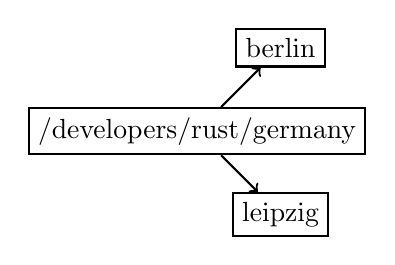
\begin{tikzpicture}[node distance={15mm}, thick, main/.style = {draw, rectangle}]
\node[main] (1) {/developers/rust/germany}; 
\node[main] (2) [above right of=1] {berlin};
\node[main] (3) [below right of=1] {leipzig}; 
\draw[->] (1) -- (2);
\draw[->] (1) -- (3);
\end{tikzpicture}
\newline

Let’s assume that each community is curated and moderated effectively on its level - relevant content is {\it added}, irrelevant content is {\it removed}.

\subsection{System}

Our proposed system consists of 3 key components:

\begin{enumerate}
    \item Data propagation mechanism
    \item Incentivization mechanism
    \item Dispute resolution mechanism.
\end{enumerate}

\subsection{Out of the scope of this paper}

For clarity these topics are left aside:
\begin{itemize}
    \item How a community is bootstrapped and updated. We assume that communities already exist in some form and there are some ways to enter or exit them
    \item How communities establish hierarchy. We assume it is easy to launch a community on top of the existing one
    \item How communities are “mirrored”. As an example: there can be many communities dedicated to Rust developers in Berlin. One of them can have such a path: {\em /developers/rust/germany/berlin} and another one can be located at path {\em /germany/berlin/developers/rust}
    \item How data is curated and sorted inside of each community. Different incentivisation mechanisms like Token Curated Registries or just a simple Reddit-like content propagation algorithm can be used to curate and sort data in the particular community
    \item How the proposed system can be automated using “auto propagation” bots or other algorithms to reduce human intervention
    \item How community members distribute rewards inside the community between its members
    \item How communities track origins of the content
    \item How communities provide Sybil-resistance
    \item How communities eliminate duplicates and normalize routes
    \item How community members are elected, especially in low level communities like "root", “earth” or “internet”.
\end{itemize}

\section{Information Propagation}
\subsection{Move Up and Move Down}

Imagine there is a “Rust Berlin 2022 conference.pdf” record in {\em berlin}'s community. Obviously it is a very specific record that is relevant only to {\em berlin}, but not relevant to {\em leipzig}.\newline

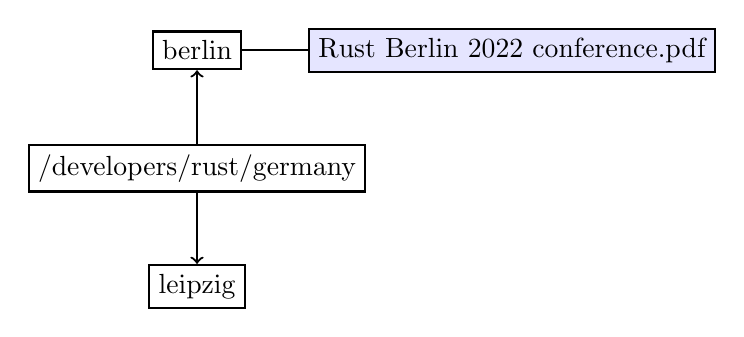
\begin{tikzpicture}[node distance={15mm}, thick, main/.style = {draw, rectangle}]
    \node[main] (1) {/developers/rust/germany}; 
    \node[main] (2) [above of=1]{berlin}; 
    \node[main] (4) [right of=2, node distance={40mm}, fill=blue!10] {Rust Berlin 2022 conference.pdf};
    \node[main] (5) [below of=1]{leipzig}; 
    \draw[->] (1) -- (2);
    \draw[-] (2) -- (4);
    \draw[->] (1) -- (5);
\end{tikzpicture}
\newline

Imagine that there is also a “Curated list of Rust meetups in Germany.pdf” record in {\em berlin}'s community.\newline

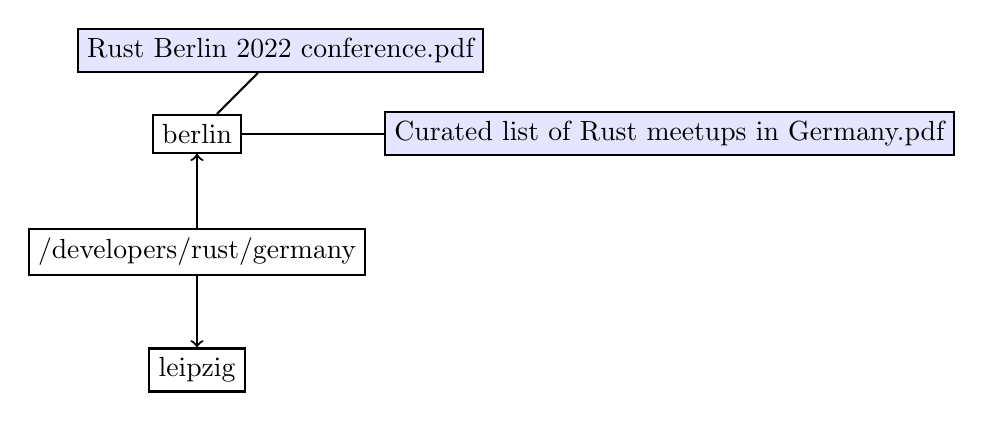
\begin{tikzpicture}[node distance={15mm}, thick, main/.style = {draw, rectangle}]
    \node[main] (1) {/developers/rust/germany}; 
    \node[main] (2) [above of=1]{berlin}; 
    \node[main] (3) [above right of=2, fill=blue!10] {Rust Berlin 2022 conference.pdf};
    \node[main] (4) [right of=2, node distance={60mm},fill=blue!10] {Curated list of Rust meetups in Germany.pdf};
    \node[main] (5) [below of=1]{leipzig}; 
    \draw[->] (1) -- (2);
    \draw[-] (2) -- (3);
    \draw[-] (2) -- (4);
    \draw[->] (1) -- (5);
\end{tikzpicture}
\newline

In this case, a record can be propagated further down to {\em germany}. Let us call this action {\it move down}. Such action can be done by either the higher level community (i.e. {\em berlin}) or by lower level community (i.e. {\em germany}).\newline

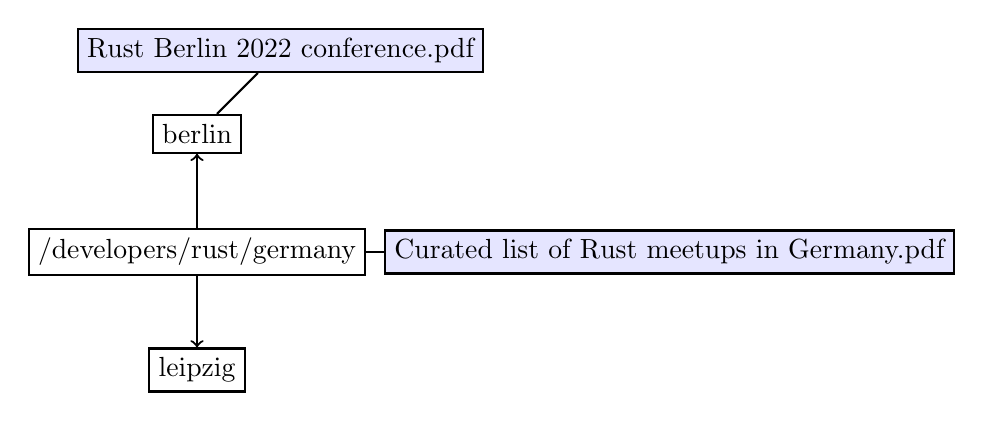
\begin{tikzpicture}[node distance={15mm}, thick, main/.style = {draw, rectangle}]
    \node[main] (1) {/developers/rust/germany}; 
    \node[main] (2) [above of=1]{berlin}; 
    \node[main] (3) [above right of=2,fill=blue!10] {Rust Berlin 2022 conference.pdf};
    \node[main] (4) [right of=1, node distance={60mm},fill=blue!10] {Curated list of Rust meetups in Germany.pdf};
    \node[main] (5) [below of=1]{leipzig}; 
    \draw[->] (1) -- (2);
    \draw[-] (2) -- (3);
    \draw[-] (1) -- (4);
    \draw[->] (1) -- (5);
\end{tikzpicture}
\newline

In some cases we will want to move data to the more specific community if it is no longer relevant. Let’s call this action {\it move up}.\newline

{\it 
Usually it is not in the interest of the higher level community to move data lower, because in this case the community will not collect incentives received by these data records (more on that later). It is only in the interest of the lower level community to collect more and more content from the top level connections. We believe that a balanced incentivization model will motivate honest and good behavior. Otherwise, if your community is bloated with erroneous or unrelated data, users will leave it.
}\newline

As a result, community members can not only {\it add}, {\it remove}, {\it hide} or {\it sort} data in their community, but also to {\it move data} to more relevant communities. This is how our curation mechanism works. And this should be reinforced with incentives. Usually extra incentives solve a problem of low user participation.\newline

Rule: community members can move data up or down one step in the hierarchy. It is not possible to move data to an arbitrary graph vertice.


\section{Multilevel Incentives}

Actions like {\it add}, {\it remove}, {\it hide} and {\it sort} should be incentivized in some way, but it is out of the scope of the current paper. However, data propagation incentives are critical for our case.

Our goal is to:

\begin{enumerate}
    \item Incentivise users to launch their community on top of existing hierarchy
    \item Incentivise community members to add relevant data to the community
    \item Incentivise more specific (higher level) community members to move data from lower level communities to increase their reward
    \item Incentivise more generic (lower level) community members to move data from top level communities to increase their reward
    \item Incentivise honest behavior.
\end{enumerate}

Different examples of incentives (also known as rewards) are as follows: tipping, payment for the paywalled contents, reputation increase, likes, global token incentives/distribution, etc.\newline

For the sake of simplicity, let’s select the first option: platform users will send tips for the interesting and relevant content.\newline

Rule: rewards should be distributed proportionally to the level in the hierarchy, from most specific to less specific communities.

\subsection{Example}

User finds a great CV in the {\em /developers/rust/germany/berlin} and wishes to send a \$1 as a tip to the {\em /berlin} community. Reward distribution is as follows:

\begin{itemize}
    \item 3\% to /
    \item 5\% to /developers
    \item 8\% to /developers/rust
    \item 13\% to /developers/rust/germany
    \item 71\% to /developers/rust/germany/berlin
\end{itemize}

Note: even if the work of adding and preparing data was done by the top level community, lower level communities still receive some percentage of fees. It is obvious that 3\% of one million tips mean huge profit for the {\em /} community. This network effect [5] will help us to bootstrap a broad hierarchy of communities with members willing to participate in the curation process.

On the other hand, it should be very easy to launch a community on top of existing one, which will force users to manually propagate information upward, which improves categorization of the data. As an example: you can create a {\em /seniors} community on top of {\em /berlin} and to move some CVs up to get more rewards.

By changing distribution rules and constants we will be able to build a balanced system in which:
being lower in the hierarchy means lower fee cut but higher inflowing stream, e.g.: 3\% of 1000000 tips.
being higher in the hierarchy means higher fee cut but lower inflowing stream, e.g.: 71\% of 100 tips.\newline

Possible improvement: in the described approach, moved data does not track the origin. This means that if content was moved from one community to another, the system will not distribute extra incentives to the original community that has added that content in the first place. This mechanism can be introduced later, but it’s outside of our scope.\newline

Possible improvement: reward rates can vary depending on how many staked tokens are locked in each community. The more tokens a community locks, the more percentage of the reward it receives. This improvement is also outside of our scope.

\subsection{What if multiple copies of data exist?}
There are three different situations in which copies of the same record can exist: 

\begin{enumerate}
    \item Copies in Unrelated communities
    \item Copies in Sibling communities
    \item Copies in Parent-child communities
\end{enumerate}

\subsubsection{Unrelated communities}
Copies exist in unrelated communities. This is totally fine as long as data is relevant to each community. Also, this situation can motivate users to create more specific communities on top of the low level hierarchy.

Example:

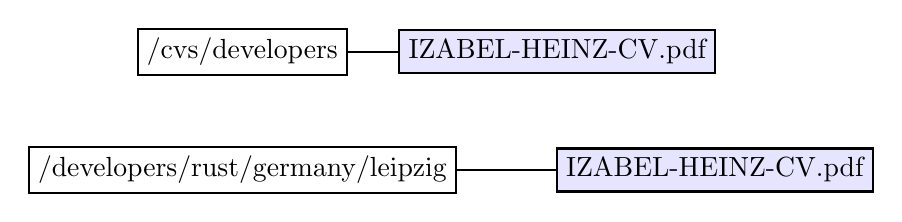
\begin{tikzpicture}[node distance={15mm}, thick, main/.style = {draw, rectangle}]
    \node[main] (1) {/cvs/developers}; 
    \node[main] (2) [below of=1]{/developers/rust/germany/leipzig}; 
    \node[main] (3) [right of=1, node distance={40mm},fill=blue!10] {IZABEL-HEINZ-CV.pdf};
    \node[main] (4) [right of=2, node distance={60mm},fill=blue!10] {IZABEL-HEINZ-CV.pdf};
    \draw[-] (1) -- (3);
    \draw[-] (2) -- (4);
\end{tikzpicture}

\subsubsection{Sibling communities}
Sibling nodes are nodes on the same hierarchical level under the same parent node. In this case data may be propagated one level down and only one copy should be left as a result. This can also be automated.

Example:

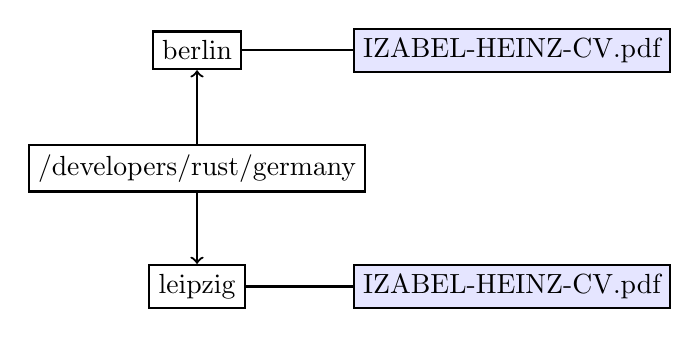
\begin{tikzpicture}[node distance={15mm}, thick, main/.style = {draw, rectangle}]
    \node[main] (1) {/developers/rust/germany}; 
    \node[main] (2) [above of=1]{berlin}; 
    \node[main] (3) [below of=1]{leipzig}; 
    \node[main] (4) [right of=2, node distance={40mm}, fill=blue!10] {IZABEL-HEINZ-CV.pdf};
    \node[main] (5) [right of=3, node distance={40mm}, fill=blue!10] {IZABEL-HEINZ-CV.pdf};
    \draw[->] (1) -- (2);
    \draw[->] (1) -- (3);
    \draw[-] (2) -- (4);
    \draw[-] (3) -- (5);
\end{tikzpicture}

\subsubsection{Parent-child communities}
Copies exist on both - parent and children levels of hierarchy. By default low level data should be selected as the correct duplicate. But the Dispute Resolution mechanism can be used if a higher level community can prove that data is more relevant and is more specific to their community.

Example:

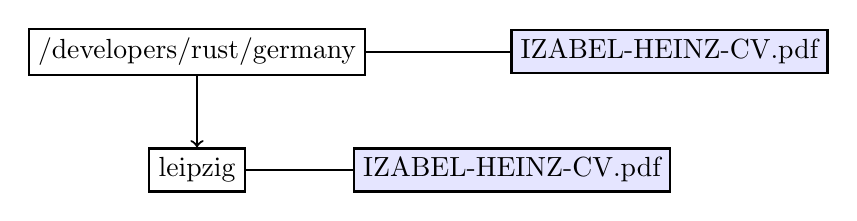
\begin{tikzpicture}[node distance={15mm}, thick, main/.style = {draw, rectangle}]
    \node[main] (1) {/developers/rust/germany}; 
    \node[main] (2) [right of=1, node distance={60mm}, fill=blue!10] {IZABEL-HEINZ-CV.pdf};
    \node[main] (3) [below of=1]{leipzig}; 
    \node[main] (4) [right of=3, node distance={40mm}, fill=blue!10] {IZABEL-HEINZ-CV.pdf};
    \draw[-] (1) -- (2);
    \draw[->] (1) -- (3);
    \draw[-] (3) -- (4);
\end{tikzpicture}

\section{Dispute Resolution}

As long as each community is incentivized with rewards, communities {\it can} try to move all data to them, in order to collect the greatest reward. We mentioned above that communities that provide data of low quality will organically get less attention by users of the system, so such a system can feature no special mechanism to prevent the adversarial behavior.

Still, we believe that a special mechanism is required. It will enforce the rules of the system and will increase the overall quality of the content on the platform.\newline

Dispute Resolution in its most simple form can be done by a moderation team run by the top-level community first. Next we will describe an approach influenced by token curated registries [2, 3]:

1 - Staking: a UserA launches a new community by submitting a staking deposit. By doing that he is now able to curate contents and move data up and down.

2 - Data propagation attempt: UserA moves some data up or down from another community.

3 - Signaling: If another UserB (not necessary from the same community) feels that action of a UserA is adversarial or wrong, she can issue a challenge, by submitting an equal amount of tokens. We call this user - a “challenger”. This initiates a voting period.

4 - Voting: Moderators then decide whether the challenger was right. There are 2 sides that moderators can take: "YES, challenger is right" or "NO, challenger is wrong".

5 - Finalizing: After the voting period concludes, tokens are settled as follows:\newline

If the challenger succeeds:
\begin{itemize}
    \item UserB receives his deposit back in full
    \item \(x\%\) of the UserA’s deposit is distributed to the UserB as a reward for winning in dispute resolution
    \item \(100-x\%\) of the UserA’s deposit is distributed to the moderators on the winning side (YES)
\end{itemize}

If the challenger fails:
\begin{itemize}
    \item UserA receives his deposit back in full
    \item \(x\%\) of the UserB’s deposit is distributed to the UserA as a reward for winning in dispute resolution
    \item \(100-x\%\) of the UserB’s deposit is distributed to the moderators on the winning side (NO)
\end{itemize}

6 - Data propagation: as an additional result of the dispute resolution process, data is finally moved to the proper community; either up or down.

\section{Conclusion}

In this work, we proposed a simple system that allows efficient data curation with the help of incentivized graphs of communities. That description should be taken into account as a simple primer of our idea. Please refer to the “out of the scope of this paper” section for more information on what components are still missing and should be considered in the real-world implementation of our idea.

\begin{thebibliography}{9}

\bibitem{murray2007}
    Murray E. Jennex,
    \textit{What is Knowledge Management?},
    \url{https://www.researchgate.net/publication/314500732_What_is_Knowledge_Management},
    2007 

\bibitem{clark2018}
    Clark R.,
    \textit{Framework-based Token Curated Registries},
    \url{https://hackernoon.com/framework-based-token-curated-registries-9691e83c2c4c},
    2018


\bibitem{goldin2017}
    Mike Goldin,
    \textit{City Walls and Bo-Taoshi: Exploring the Power of Token-Curated Registries},
    \url{https://medium.com/@ilovebagels/token-curated-registries-1-0-61a232f8dac7},
    2017

\bibitem{yuezhou2015}
    Yuezhou Lv, Thomas Moscibroda,
    \textit{Incentive Networks},
    \url{https://www.microsoft.com/en-us/research/wp-content/uploads/2016/02/AAAI_2015.pdf},
    2015

\bibitem{networkEffect}
    \textit{Wikipedia: Network Effect},
    \url{https://en.wikipedia.org/wiki/Network_effect}

\end{thebibliography}

\end{document}
